\documentclass[14pt]{extbook}
\usepackage{multicol, enumerate, enumitem, hyperref, color, soul, setspace, parskip, fancyhdr} %General Packages
\usepackage{amssymb, amsthm, amsmath, bbm, latexsym, units, mathtools} %Math Packages
\everymath{\displaystyle} %All math in Display Style
% Packages with additional options
\usepackage[headsep=0.5cm,headheight=12pt, left=1 in,right= 1 in,top= 1 in,bottom= 1 in]{geometry}
\usepackage[usenames,dvipsnames]{xcolor}
\usepackage{dashrule}  % Package to use the command below to create lines between items
\newcommand{\litem}[1]{\item#1\hspace*{-1cm}\rule{\textwidth}{0.4pt}}
\pagestyle{fancy}
\lhead{Progress Quiz 5}
\chead{}
\rhead{Version B}
\lfoot{9912-2038}
\cfoot{}
\rfoot{Spring 2021}
\begin{document}

\begin{enumerate}
\litem{
What is the domain of the function below?\[ f(x) = \sqrt[5]{4 x - 3} \]\begin{enumerate}[label=\Alph*.]
\item \( \text{The domain is } [a, \infty), \text{   where } a \in [0.64, 0.99] \)
\item \( \text{The domain is } (-\infty, a], \text{   where } a \in [0.01, 0.94] \)
\item \( \text{The domain is } [a, \infty), \text{   where } a \in [1.1, 1.66] \)
\item \( (-\infty, \infty) \)
\item \( \text{The domain is } (-\infty, a], \text{   where } a \in [1.23, 2.25] \)

\end{enumerate} }
\litem{
Choose the graph of the equation below.\[ f(x) = \sqrt{x - 6} + 3 \]\begin{enumerate}[label=\Alph*.]
\begin{multicols}{2}\item 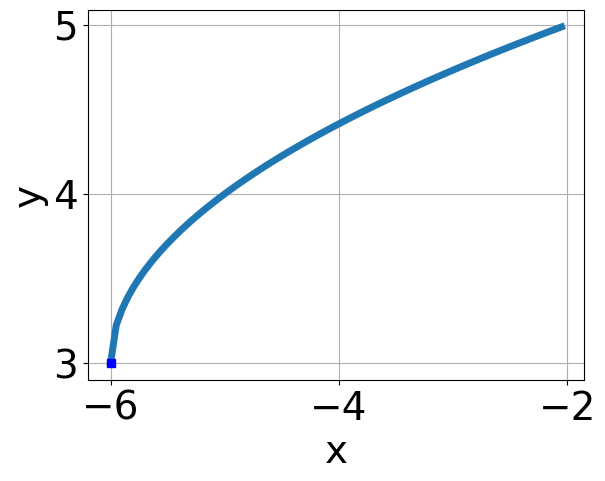
\includegraphics[width = 0.3\textwidth]{../Figures/radicalEquationToGraphAB.png}\item 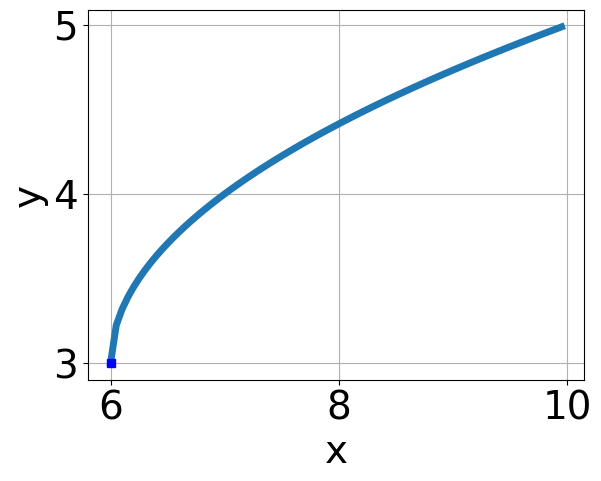
\includegraphics[width = 0.3\textwidth]{../Figures/radicalEquationToGraphBB.png}\item 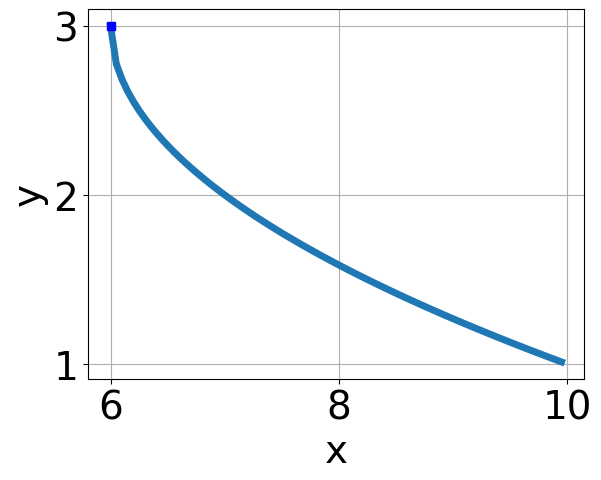
\includegraphics[width = 0.3\textwidth]{../Figures/radicalEquationToGraphCB.png}\item 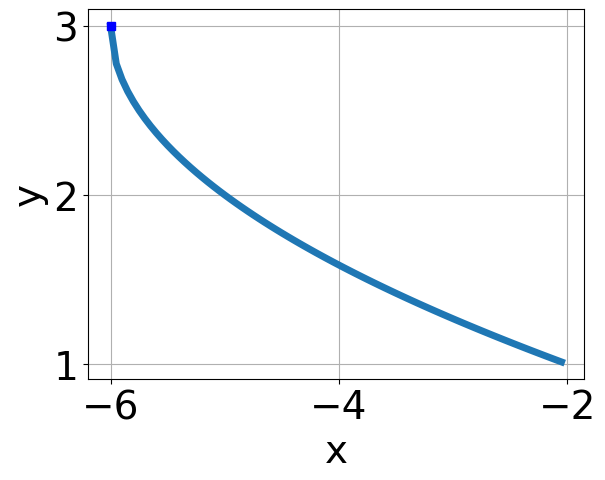
\includegraphics[width = 0.3\textwidth]{../Figures/radicalEquationToGraphDB.png}\end{multicols}\item None of the above.
\end{enumerate} }
\litem{
Solve the radical equation below. Then, choose the interval(s) that the solution(s) belongs to.\[ \sqrt{7 x - 5} - \sqrt{9 x - 8} = 0 \]\begin{enumerate}[label=\Alph*.]
\item \( x \in [1.11,1.73] \)
\item \( x \in [-6.75,-6.14] \)
\item \( x_1 \in [-0.28, 1.29] \text{ and } x_2 \in [1.19,1.6] \)
\item \( \text{All solutions lead to invalid or complex values in the equation.} \)
\item \( x_1 \in [-0.28, 1.29] \text{ and } x_2 \in [0.66,0.91] \)

\end{enumerate} }
\litem{
Solve the radical equation below. Then, choose the interval(s) that the solution(s) belongs to.\[ \sqrt{-35 x^2 - 49} - \sqrt{84 x} = 0 \]\begin{enumerate}[label=\Alph*.]
\item \( x_1 \in [-1.85, -1.38] \text{ and } x_2 \in [-1.1,0] \)
\item \( x_1 \in [0.88, 1.92] \text{ and } x_2 \in [0.6,4.4] \)
\item \( \text{All solutions lead to invalid or complex values in the equation.} \)
\item \( x \in [-1.06,-0.59] \)
\item \( x \in [-1.85,-1.38] \)

\end{enumerate} }
\litem{
Solve the radical equation below. Then, choose the interval(s) that the solution(s) belongs to.\[ \sqrt{9 x - 8} - \sqrt{7 x - 6} = 0 \]\begin{enumerate}[label=\Alph*.]
\item \( x_1 \in [0.87, 0.94] \text{ and } x_2 \in [0.95,1.05] \)
\item \( x_1 \in [0.72, 0.86] \text{ and } x_2 \in [0.79,0.98] \)
\item \( x \in [6.99,7.07] \)
\item \( x \in [0.98,1.06] \)
\item \( \text{All solutions lead to invalid or complex values in the equation.} \)

\end{enumerate} }
\litem{
Choose the graph of the equation below.\[ f(x) = \sqrt{x + 10} - 4 \]\begin{enumerate}[label=\Alph*.]
\begin{multicols}{2}\item 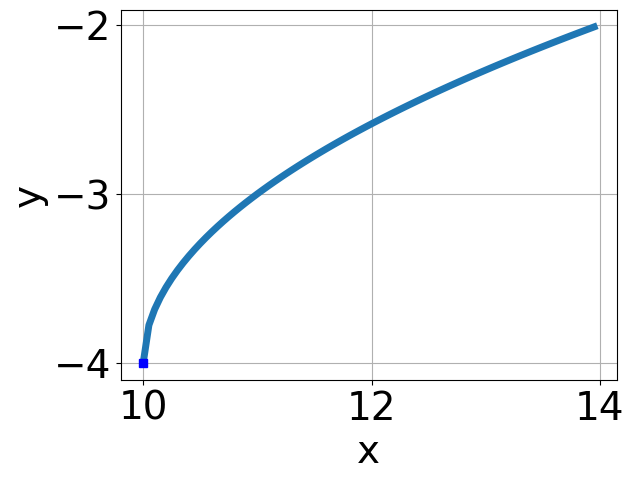
\includegraphics[width = 0.3\textwidth]{../Figures/radicalEquationToGraphCopyAB.png}\item 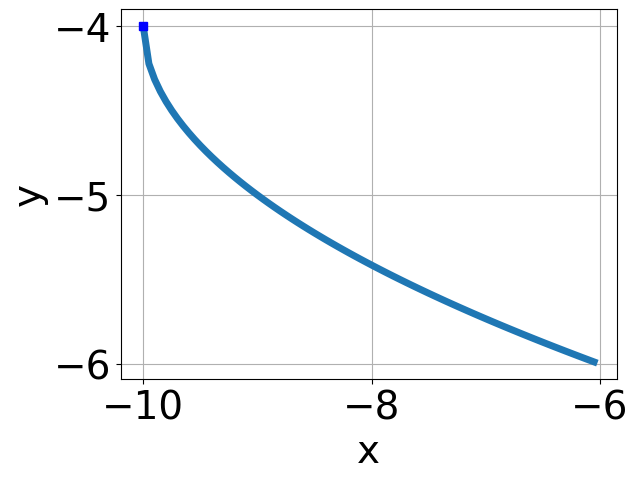
\includegraphics[width = 0.3\textwidth]{../Figures/radicalEquationToGraphCopyBB.png}\item 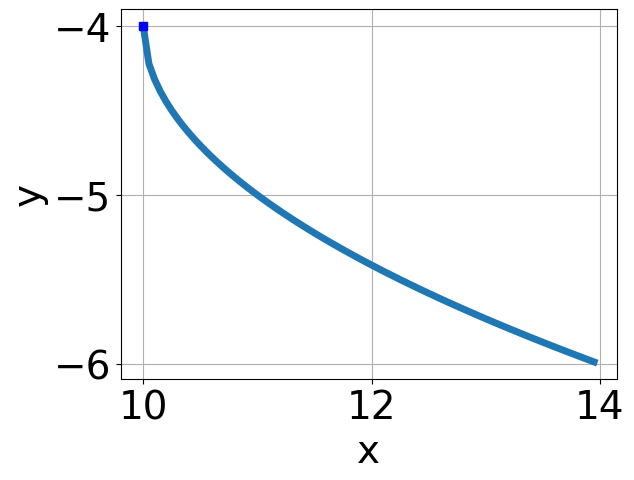
\includegraphics[width = 0.3\textwidth]{../Figures/radicalEquationToGraphCopyCB.png}\item 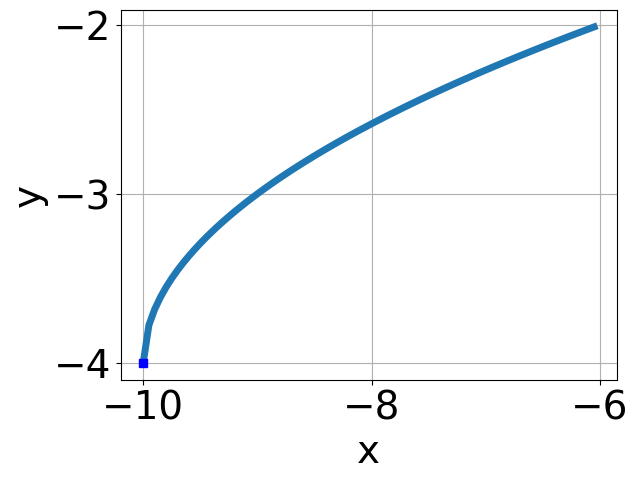
\includegraphics[width = 0.3\textwidth]{../Figures/radicalEquationToGraphCopyDB.png}\end{multicols}\item None of the above.
\end{enumerate} }
\litem{
Choose the equation of the function graphed below.
\begin{center}
    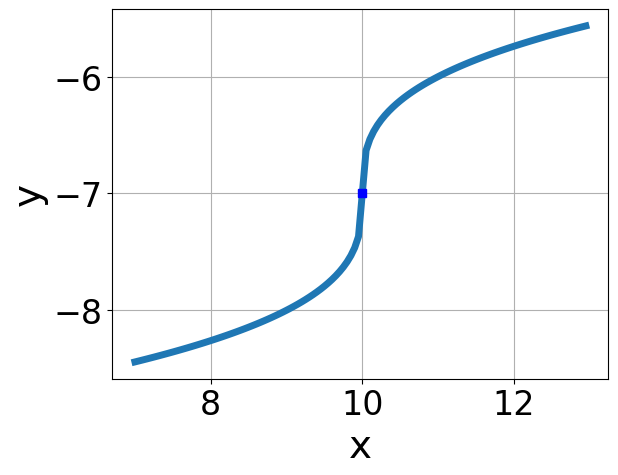
\includegraphics[width=0.5\textwidth]{../Figures/radicalGraphToEquationCopyB.png}
\end{center}
\begin{enumerate}[label=\Alph*.]
\item \( f(x) = - \sqrt{x - 10} - 7 \)
\item \( f(x) = \sqrt{x + 10} - 7 \)
\item \( f(x) = \sqrt{x - 10} - 7 \)
\item \( f(x) = - \sqrt{x + 10} - 7 \)
\item \( \text{None of the above} \)

\end{enumerate} }
\litem{
Solve the radical equation below. Then, choose the interval(s) that the solution(s) belongs to.\[ \sqrt{-28 x^2 - 72} - \sqrt{-95 x} = 0 \]\begin{enumerate}[label=\Alph*.]
\item \( x \in [-1.1,1.3] \)
\item \( x_1 \in [-1.3, 0.7] \text{ and } x_2 \in [-4.25,-1.25] \)
\item \( x_1 \in [-1.1, 1.3] \text{ and } x_2 \in [2.25,4.25] \)
\item \( \text{All solutions lead to invalid or complex values in the equation.} \)
\item \( x \in [1.8,4.3] \)

\end{enumerate} }
\litem{
What is the domain of the function below?\[ f(x) = \sqrt[6]{-7 x - 4} \]\begin{enumerate}[label=\Alph*.]
\item \( [a, \infty), \text{where } a \in [-3.9, -1] \)
\item \( (-\infty, a], \text{ where } a \in [-1.2, 1] \)
\item \( [a, \infty), \text{where } a \in [-1, 0.6] \)
\item \( (-\infty, a], \text{where } a \in [-3.3, -0.6] \)
\item \( (-\infty, \infty) \)

\end{enumerate} }
\litem{
Choose the equation of the function graphed below.
\begin{center}
    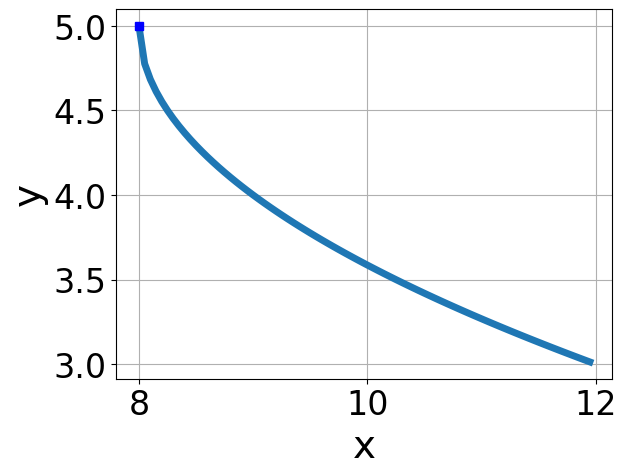
\includegraphics[width=0.5\textwidth]{../Figures/radicalGraphToEquationB.png}
\end{center}
\begin{enumerate}[label=\Alph*.]
\item \( f(x) = \sqrt[3]{x + 8} + 5 \)
\item \( f(x) = - \sqrt[3]{x - 8} + 5 \)
\item \( f(x) = - \sqrt[3]{x + 8} + 5 \)
\item \( f(x) = \sqrt[3]{x - 8} + 5 \)
\item \( \text{None of the above} \)

\end{enumerate} }
\end{enumerate}

\end{document}